\chapter{Benchmark implementation}

The design of the benchmark overhead leads directly to its implementation. The
benchmark functionality, written in TypeScript, involves two main components:
the \texttt{BenchmarkRunner} and \texttt{BenchmarkSuite} classes. The classes
work together to manage the ordering of tests, database administration, and
execution of test suites, as well as handling packages, test suites, and
reporters.


\begin{figure}[h]
    \caption{Simplified schema of the Benchmark class architecture}
    \centering
    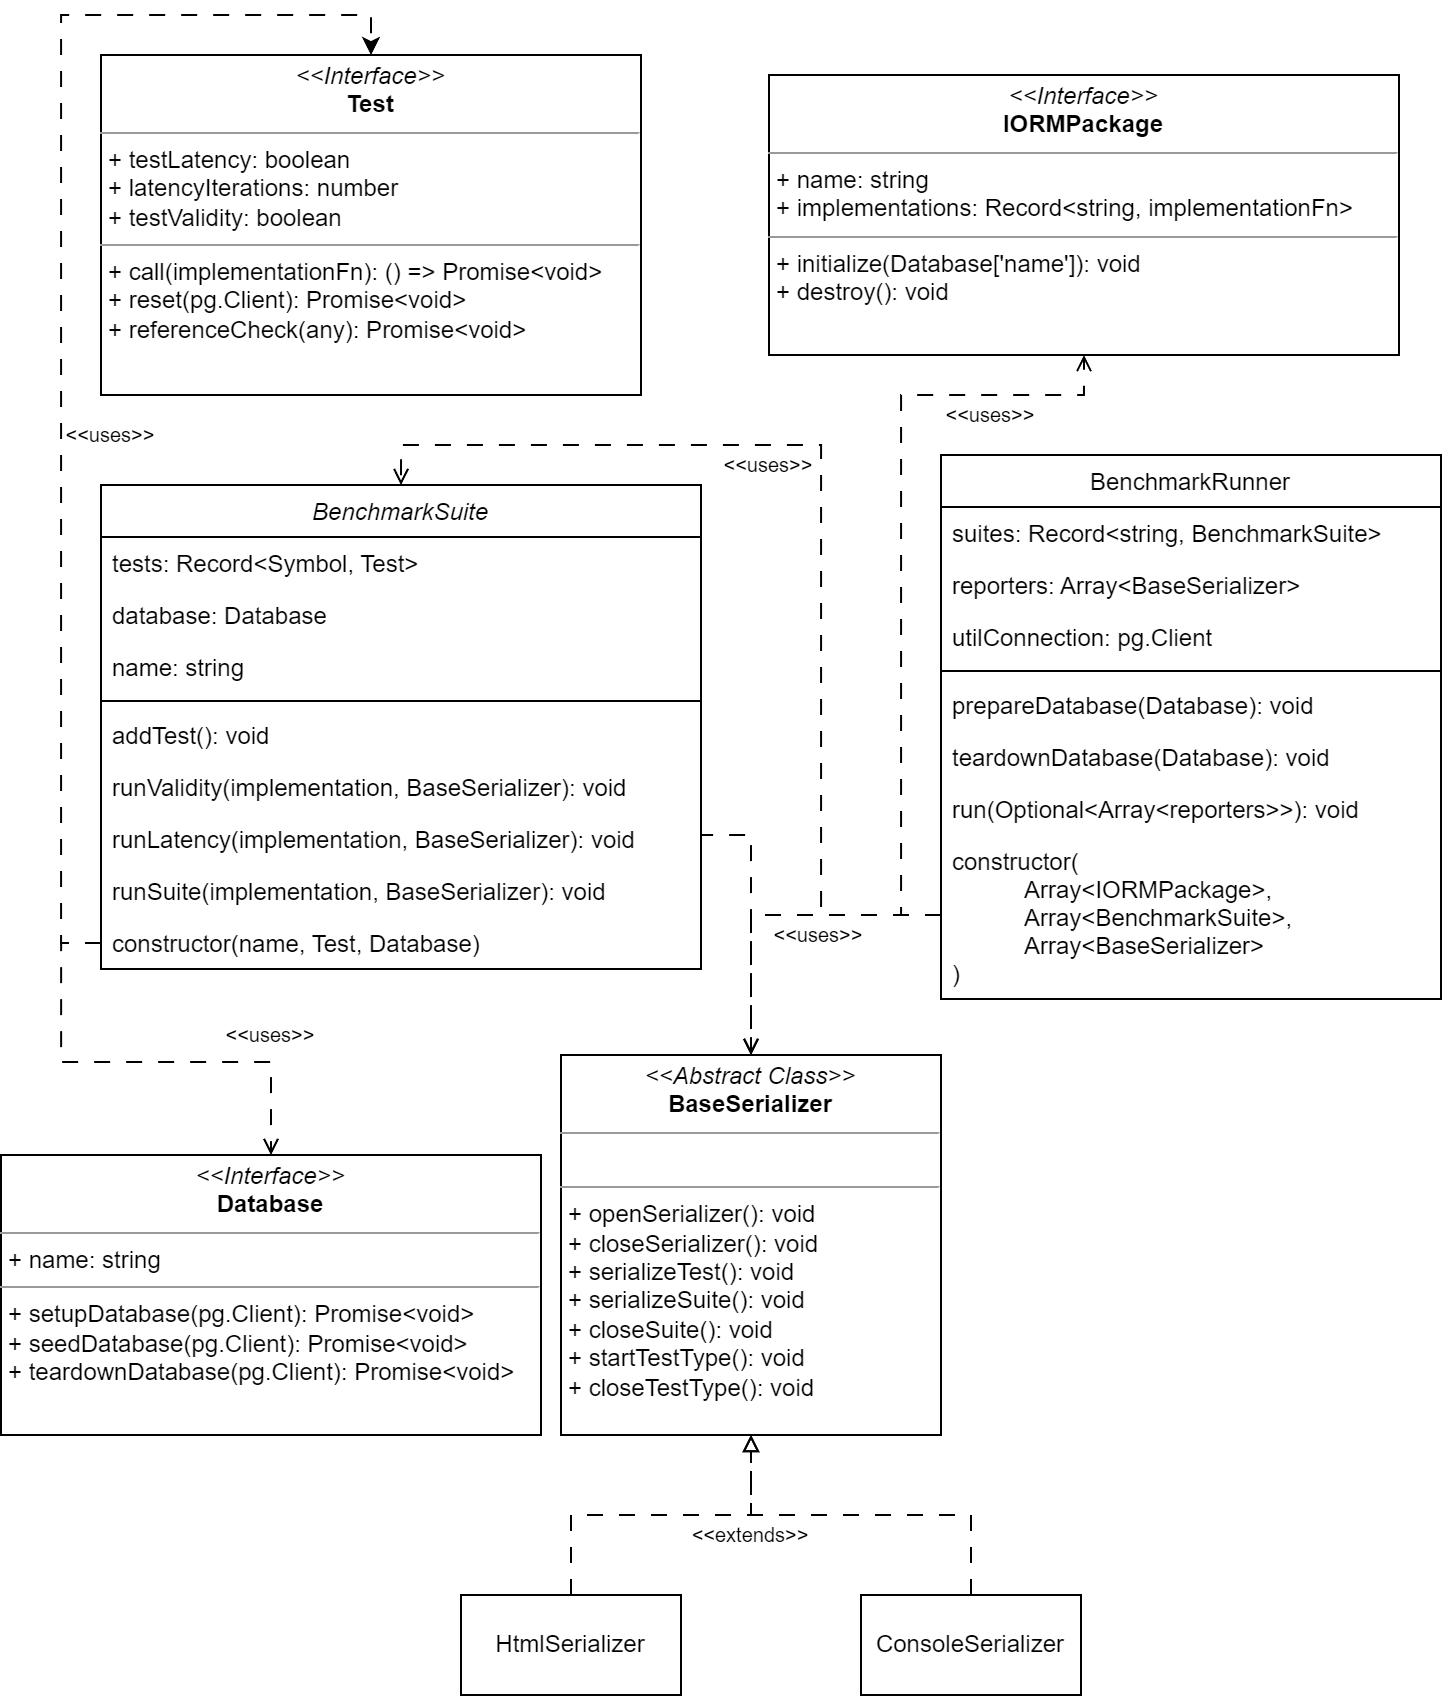
\includegraphics[width=\textwidth]{BenchmarkClasses}
\end{figure}

\section{BenchmarkRunner}

The \texttt{BenchmarkRunner} class is responsible for managing the benchmark’s
overall execution. It holds information about the test suites, ORM and query
builder packages being tested, and the reporters. The class has responsibility
for database administration while also ordering and executing the test suites on
their respective database schemas.

Database administration tasks include setting up and tearing down example
databases used in testing. Tests are currently written only for the database
examined in chapter \ref{ch:database}, therefore this functionality is only used
to initialize the database to preserve a consistent state. In order to perform
these tasks, \texttt{BenchmarkRunner} maintains its database connection using
the default \texttt{pg} module.

The benchmark runner is also responsible for ordering, initialization and
execution of individual packages and tests. Each package is declared using a
unified interface, which defines initialization and destruction methods for
efficient memory usage, implemented test suites and package name. The order of
executions is guided by the database schema selected, the package, and
individual test suites. If any suites are not implemented in the individual
package declaration, the reporters are notified, and the tests can be marked as
not implemented in the report.

\section{BenchmarkSuite}

As the name suggests, \texttt{BenchmarkSuite} represents each test suit of the
benchmark. It covers the specification of each test, including validation
function, name, parameters and options for running the test. This design ensures
type safety for running the tests as they implement the interface defined for
the suite. The options include which tests should be performed or how many loops
to execute for repeated tests. Class methods implement individual types of
tests, error handling for individual runs and measuring the execution time of
each test run.

Two implemented test workflows, validity test and latency test; validity test
runs each implementation once, tests if the value is equal to reference in both
value and the runtime type and returns test result. The latency test executes
the tests in a loop, intending to show if the framework can create well-crafted
queries without adding significant overhead.

\section{Reporters}
As the output of the benchmarks is meant to be interpreted by humans, the
measured data needs to be transformed into a human-readable format. Test objects
contain vital information, but the benchmark output consists of thousands of
such objects; therefore, they must be converted into valuable data. Two
reporters were implemented for this benchmarking framework, with an interface
for further reporters.

\subsection{Console Reporter}
The primary reporter for use in development intends to provide simple benchmark
results in table form. While running the benchmark, it allows for quick
assessment of any errors and monitors the progress of the run.

\subsection{HTML Reporter}
The HTML reporter is the primary source for any data analysis of the benchmark
run. It consists of a template file and the reporter. The reporter receives data
from the benchmark using the unified API, parses it, and inserts it into the
template file as a JSON string once the benchmark is finished. Along with the
data, cascading style sheets are also inserted, as they are written in
\texttt{Sass} language \cite{Sass}, which must be compiled before the HTML file
viewer uses them. After the template is completed, the file is saved separately,
and graphs are created on runtime using JavaScript.

While the data could be served dynamically, this separate file allows for
multiple runs to be saved and be independent of the server which would provide
the data. The JSON is available and can be inspected if further analysis is
needed.

\section{Benchmarks}
This section will list and describe all the benchmarks developed to compare
individual packages. In addition to comparing performance, the requirements for
implementation are comparison, as an easily implemented framework is better than
one that's difficult to, provided they both perform similarly.

\subsection{MVP Benchmark}
This test suite was only implemented under the \textit{Knex.js} package as its
purpose is to test the functionality of the benchmarking framework and does not
test any database functionality. It is proof of concept for correct validation
and exception handling tests for the benchmark suite and runner implementation.
It consists of a small number of tests, including a fully passing test, a test
expecting \texttt{Skipped} exception, which is used for marking tests which are
not implemented, tests whose results are mismatched in value or runtime type,
and a test that throws generic error on execution. Additionally, MVPBench
examines if test configurations are working as they should be, testing both
validity and latency settings.

\subsection{Entity Traversal Benchmark}
One of the generally provided functionalities of ORMs is the ability to define
entities and their relations. This benchmark aims to test the ability to use
these defined relations to find objects using these connections. The first test
of the suit focuses on finding a cat's colour in hex by traversing two
relations, one of which is identifying. The framework starts with the cat's ID
and needs to fetch the \texttt{color\_hex} instance through its connection to
the \texttt{cat\_color} instance. Thanks to the relation design, there is a
guarantee that only one result will be returned at any time. The second test
counts cats by their colour hex code, traversing the relations from the first
test in the opposite direction. Instead of selecting, the test counts the cats,
testing if the query difficulty changes if we use aggregate functions instead of
basic \texttt{SELECT} query. The third test in this benchmark selects all toys
available to a cat, primarily focusing on the format of the returned data and
how well the decomposition table can be accessed or avoided. The decomposition
table exists because of the M:N relation between toys and houses, but the
additional amount attribute is not used.

\subsection{Edge Cases Benchmark}

The edge cases benchmark aims to evaluate database adapter performance in
specific situations that may not be commonly encountered but can potentially
cause problems. The two tests in this benchmark focus on data type conversion
and parameter handling.

BigIntColumn test examines the data type conversion for the BigInteger type in
PostgreSQL. JavaScript's Number type can lose precision when handling large
integers since the maximum safe integer for Number is \(2^{53} - 1\)
\cite{MDNNumber}, while PostgreSQL's \texttt{bigint} type can store numbers up
to \(2^{63} - 1\) \cite{PostgresNumeric}. Although the BigInt primitive
\cite{MDNBigInt}, which can store integers with arbitrary precision, was
introduced in ECMAScript 2020 (ES11) \cite{ecma-262} and has been implemented in
Node.js since 2018 \cite{MDNBigInt}, not all frameworks handle this type
correctly. The frameworks can either cast the value to Number, losing precision
and failing the test, or return the value as a string or, ideally, as a BigInt
primitive.

SQL Injection test assesses the framework's basic handling of parameters. One of
the main reasons for using a database access package over a basic driver is to
improve security against SQL injection attacks. The code will return all records
if the parameter is sent as part of the SQL query. If the package incorrectly
escapes the query, it will result in no results returned. Only the correct
handling of arguments will return the specific Cat with the fascinating name a
\enquote{\texttt{' or true --}}. It is important to note that this test does not
evaluate whether the package is entirely vulnerable to SQL injection attacks but
rather if the basic handling of arguments is not vulnerable.

\subsection{Special SQL Actions Benchmark}

The Special SQL Actions benchmark evaluates the performance of frameworks in
scenarios that go beyond basic querying, focusing on unique ways of interacting
with the database. This benchmark comprises several tests, each targeting
different aspects of database interactions.

The \textit{upsertToysToHouse} test examines whether the package contains an
upsert operation method and assesses its flexibility, such as the ability to
differentiate between the insertion and update objects, as well as the capacity
to reference the updated value. The test uses a CatDatabase schema that includes
a decomposition table called ToysHouse, which stores references between houses
and toys and the quantity of each toy type in the house.

The suite also contains tests which evaluate the handling of JSON columns in the
database. The \textit{JSONColumn} test checks the ability to parse JSON values
from the database, while the \textit{JSONWhere} test focuses on querying based
on the value of an object key inside the JSON column. PostgreSQL provides two
ways to query the value: extraction operator \texttt{->>} for simple comparisons
or \texttt{@>} operator for more complex comparisons with JSONB datatype
\cite{postgres-json}, which are useful for developers using SQL, but the
abstraction of ORM might remove the access to these methods.

The \textit{transactionalOperations} test investigates how individual packages
handle transactions, assessing the full range of operations available for
reverting changes to the data.

Lastly, the \textit{likeQuery} test examines the methods each framework uses for
pattern-matching queries, evaluating basic search functionality in the database
by searching for a part of a house address.

By understanding how different frameworks handle these particular SQL actions,
developers can make informed decisions when selecting a database adapter that
aligns with their project's unique requirements. The benchmark ensures that
developers are aware of each package's various capabilities and limitations,
enabling them to choose the most suitable solution for their specific use cases.